\section{Getting Started}

\htmlmenu{2}

\newcommand{\myimg}[1]{\texorhtml{\includegraphics[width=5mm]{../images/#1}}{\htmlimg{../images/#1}}\ }

To get started, use the File $\rightarrow$ Open menu, and load the
simulation world file \texttt{dlr\_flask.wld}. Note that by default
GraspIt!  will look for world files in \texttt{\$GRASPIT/worlds}. This
is a very simple simulation world containing nothing except a hand
(the DLR model) and an object (a flask).

\begin{figure}[h]
\texorhtml{
\centerline{
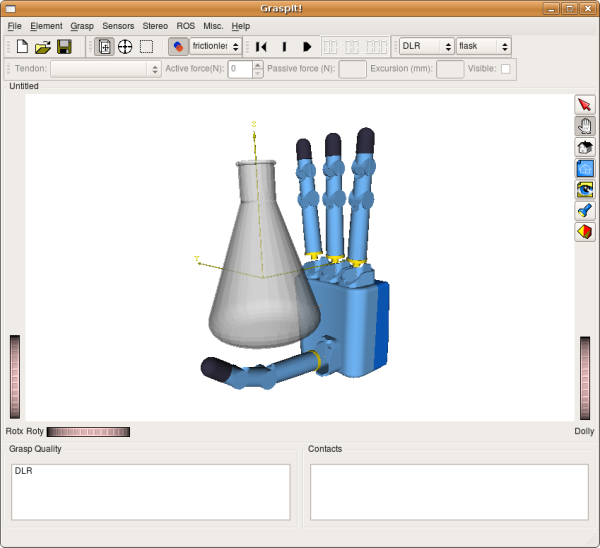
\includegraphics[width=5.0in]{../images/dlr_flask.png}}
}
{\htmlimg{../images/dlr_flask.png}
}
\end{figure}

In general, you can also start with an empty simulation world and
populate it by importing robots and objects, one at a time, using the
Import options in the File menu. You can then save a simulation world
into a world file, like the one that we just opened. In this quick
tutorial, we will be using a couple of simulation worlds supplied with
the distribution.

\subsection{The main window and controls}

The most part of the GraspIt! main window is occupied by the Inventor
viewer, which renders the virtual world. On the right side there is a
vertical toolbar: this is the Inventor toolbar which is responsible
for camera interaction.

The first two buttons on the Inventor toolbar determine which state
the viewer is in. When \myimg{arrowTool.jpg} is selected, the viewer
is in \textbf{Interaction mode}. This is the only mode in which you
can interact with the objects in the simulation world. When
\myimg{handTool.jpg} is selected, the viewer is in \textbf{Camera
  mode}. This is the only mode in which you can move the camera.

You can also toggle between \textbf{Interaction mode} and
\textbf{Camera mode} by pressing the \texttt{<ESC>} or \texttt{<ALT>}
keys, although this seems not to work on all systems.

\subsubsection{The Camera mode}

When the viewer is in \textbf{Camera mode}, you can move the virtual
camera in the following ways:
\begin{itemize}
\item \textbf{Rotate} - Hold down the left mouse button and drag;
\item \textbf{Translate} - Hold down \texttt{<CTRL>} and the left
  mouse button and drag; alternatively, hold down the middle mouse
  button and drag;
  \item \textbf{Zoom} - Hold both the left and middle mouse buttons
    and drag, or rotate the wheel on a wheel mouse.
\end{itemize}

In addition, the following buttons on the Inventor toolbar are useful:
\begin{itemize}
\item \myimg{viewAllTool.jpg} - This automatically moves the camera so
  that the entire scene fits in the viewer window;
\item \myimg{seekTool.jpg} - The seek tool allows you to click on an
  object in the scene. After you click, the camera zooms in on the
  object, which also becomes the center of rotation.
\end{itemize}

Take a moment to move the camera around and familiarize yourself with
its controls.

\subsubsection{The Interaction mode}

When the viewer is in \textbf{Interaction mode}, you can interact with
the objects in the scene. The type of interaction is determined by the
following button in the GraspIt! toolbar: \myimg{translateTool.jpg}
\myimg{rotateTool.jpg} \myimg{selectTool.jpg}:

\begin{itemize}
\item \myimg{translateTool.jpg} - \textbf{Translate or set
  joints}. Clicking on a body or the base (palm) of a robot causes a
  box to be drawn around it. This box acts as a translation
  manipulator. By clicking on the sides of the box and dragging the
  mouse, the body or robot can be translated in 2 dimensions that are
  aligned with the face of the box that was clicked. Holding down
  \texttt{<SHIFT>} constrains this motion to one axis. If a robot is
  selected and moved.

  Clicking on a kinematic chain causes joint draggers to be drawn for
  each DOF on that chain. You can then use these draggers to move the
  joints of the robot.
\item \myimg{rotateTool.jpg} - \textbf{Rotate}. Clicking a body or
  robot base link brings up a spherical rotation manipulator. Dragging
  the ball allows rotation of the selected item in three
  dimensions. By clicking one of the stripes, the body can be rotated
  about one axis at a time. By dragging the cross hairs, the ball can
  be re-centered to rotate about a different point. The limitations
  concerning connected robots applies to rotation as well.
\item \myimg{selectTool.jpg} - \textbf{Select}. Clicking a body will
  select it, and this is indicated with a wireframe overlay. Holding
  down \texttt{<SHIFT>} allows multiple bodies to be selected, or
  clicking on an already selected link of a robot will select the
  whole robot. Once a body (or bodies) has been selected, its
  collision and material properties are shown in the next part of the
  toolbar. They can then be changed or additional properties can be
  changed using the menu item described below. After a body is
  selected, the user may remove the body from the world by pressing
  \texttt{<DEL>}.
\end{itemize}

Try to use the \myimg{translateTool.jpg} tool to flex the fingers of
the robot. Note that once a finger touches the object, a contact is
marked and no more flexion is allowed. The same behavior applies for
moving objects or robots around.

The following buttons in the GraspIt! toolbar apply to the currently
selected body (if any):
\begin{itemize}
\item \myimg{collide.jpg} - \textbf{Toggle Collisions}. There are 3
  different ways to use this property:
\begin{itemize}
\item if no body is selected, this button allows collision checking
  for the entire world to be switched on or off.
\item if one or more than two bodies are selected, this button sets
  the collision checking for those bodies. A body that has collision
  checking turned off can pass through ANY other body.
\item if two bodies are selected, this button allows collision
  checking between ONLY that pair of bodies to be disabled.
\end{itemize}
\item \myimg{materialSelect.jpg} - \textbf{Material}. This sets the
  material for the selected bodies, which affects the coefficient of
  friction when contacts arise.
\end{itemize}

Try to disable collisions for the entire simulation world. Note that
now you can move objects or flex fingers freely, even if that results
in a collisions. Make sure you move all objects out of collisions
\textbf{before} you re-enable collision checking; otherwise, you will
not be able to move them around.

You can also create one or more contacts between the hand and the
object. Once you have a contact, select one of the bodies in contact
(such as the robot link that is touching the flask, or the flask
itself) and change its material. Notice how the friction cone that
marks the contact changes as well.

\subsection{Grasp example}

Start by loading the simulation world \texttt{dlr\_flask.wld} again,
to make sure all the world elements are in their original
positions. The use the menu Grasp $\rightarrow$ Auto Grasp. This will cause all
the fingers of the robot to flex (more details can be found in the
\link*{robot configuration file}{sec:robotfile}) until contact with
the flask prevents all further motion. You now have a grasp.

Use the Grasp $\rightarrow$ Quality Measures... menu to create a new quality
measure that will be used on this grasp. By default, the quality
measure dialog that appears will create a new quality measure called
\textbf{New Quality Measure} of the \textbf{Epsilon} type using an L1
Grasp Wrench Space. Click \textbf{Add/Edit}, and then click
\textbf{OK}. The new quality measure, along with its value, will be
displayed in the lower left part of the GraspIt! main window.

You can also create a projection of the Grasp Wrench Space for this
grasp. Use the Grasp $\rightarrow$ Create GWS Projection menu. Then click the
three checkboxes marked \textbf{tx, ty} and \textbf{tz} and click
\textbf{OK}. GraspIt! will display the space of forces that this grasp
can apply without a net torque. Note that if you change the camera in
the main GraspIt! viewer, the camera that shows the GWS projection
moves as well. The axes of the GWS projection are always aligned with
the axes of the main viewer.

\subsection{Dynamics example}

Start by loading the simulation world
\texttt{barrettGlassDyn.wld}. Then, start the dynamics engine by
pressing the \myimg{play.jpg} button on the Dynamics toolbar. Note
that the robot joints move slightly and the glass slowly rolls on the
table. The PD controllers in the robot joints are simply maintaining
the current position against gravity.

Use the Grasp $\rightarrow$ Auto Grasp menu to close the fingers of the
hand. Note that the hand starts closing, then lifts the glass into its
grasp. After the grasp stabilizes, select the glass and change its
material properties to \texttt{frictionless}. The glass then slips out
of the grasp and ends up rolling off the table. You can pause the
dynamics engine at any time by clicking the pause button in the
dynamics toolbar.

\subsection{The menus}

Here is a subset of the functionality in the menus (I hope to update
this section soon):

\begin{itemize}
\item \textbf{File Menu}
\begin {itemize}
\item \textbf{New} Empties the current world and resets the simulation time.
\item \textbf{Open...}  Loads a new world configuration.
\item \textbf{Save, Save As...}  Saves the current world
  configuration. Velocities are not saved.
\item \textbf{Save Image...}  Renders the scene using the current
  camera and saves the image in jpg format. The image will be
  antialiased.
\item \textbf{Import Robot...}  Loads a robot from a robot
  configuration file and places it at the world origin. After
  importing a robot or body, click view all if the imported object
  does not fit in the viewer.
\item \textbf{Import Object...}  Loads an Inventor model and places it
  in the world as a graspable body. The Inventor file must have mass
  and material defined in the comments. The body is made transparent
  so that contacts can be seen.
\item \textbf{Import Obstacle...}  Loads an Inventor model and places
  it as a static object in the world. These objects may be moved by
  the user but their motions are not computed during dynamic
  simulation.
\item \textbf{Edit Settings...}  Allows the user to change persistant
  program settings. The settings are stored in the registry in
  Windows, and in an rc file in Linux. See below for a description of
  this dialog box.
\item \textbf{Exit} Exits the program.
\end{itemize}
\item \textbf{Element}
\begin{itemize}
\item \textbf{Translate} Same as translate toolbar button. See above.
\item \textbf{Rotate} Same as rotate toolbar button. See above.
\item \textbf{Select} Same as select toolbar button. See above.
\item \textbf{Collisions ON/OFF} Same as collision toggle toolbar
  button. See above.
\item \textbf{Body Properties...}  Brings up a dialog box that allows
  the user to edit the properties of the currently selected
  bodies. See below for a description of this dialog box.
\end{itemize}
\item \textbf{Grasp}
\begin{itemize}
\item \textbf{Auto Grasp} Starts an auto-grasp. When the dynamics are
  not running, this closes the fingers of a hand until joint limits
  are reached or contacts prevent further motion. The relative
  velocity of the joints is defined in the robot configuration
  file. When dynamics are running, a trajectory generator will create
  a position trajectory that will close the fingers. The joint
  controllers will then use these positions as set points and adjust
  the joint forces.
\item \textbf{Create GWS Projection...}  Opens a dialog box to allow
  the user to choose a projection of the 6D grasp wrench space. After
  the projection is chosen, GraspIt! opens a new window showing the
  projected wrench space. The volume is updated each time the grasp
  changes.
\item \textbf{Quality Measures...}  Allows the user to create a new
  quality measure that will be evaluated each time the grasp
  changes. (More documentation on this soon.)
\item \textbf{Planner...}  Opens a dialog box containing settings for
  the automatic grasp planner. At this time this only works with the
  Barrett hand.
\end{itemize}
\end{itemize}
